% !TeX root = Thesis.tex

\begin{figure}[ht]
    \centering
    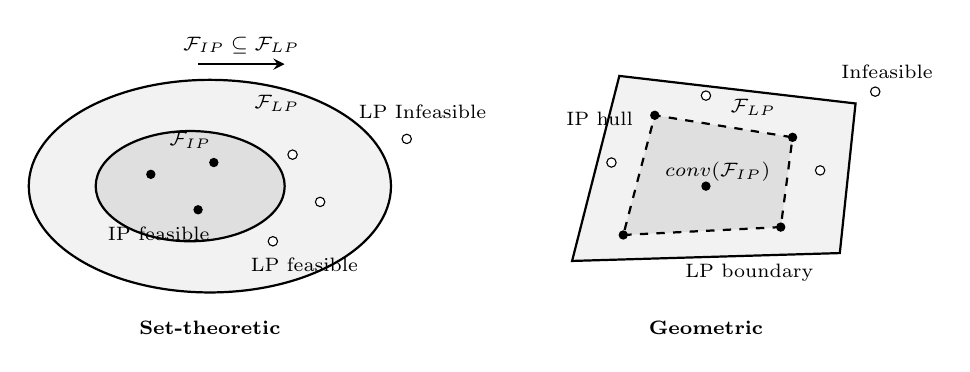
\begin{tikzpicture}[
        >=stealth,
        every node/.style={font=\scriptsize},
        feasible/.style={circle,fill=black,inner sep=1.2pt},
        fractional/.style={circle,fill=white,draw=black,inner sep=1.2pt},
        infeasible/.style={circle,fill=white,draw=black,inner sep=1.2pt}
    ]

    \begin{scope}
        \draw[thick,fill=gray!10] (0,0) ellipse (2.3cm and 1.35cm);
        \draw[thick,fill=gray!25] (-0.25,0) ellipse (1.2cm and 0.7cm);
        \node[feasible] at (-0.75,0.15) {};
        \node[feasible] at (0.05,0.3) {};
        \node[feasible] at (-0.15,-0.3) {};
        \node[fractional] at (1.05,0.4) {};
        \node[fractional] at (1.4,-0.2) {};
        \node[fractional] at (0.8,-0.7) {};
        \node[infeasible] at (2.5,0.6) {};
        \node at (0.85,1.05) {$\mathcal{F}_{LP}$};
        \node at (-0.25,0.58) {$\mathcal{F}_{IP}$};
        \node at (-0.65,-0.6) {IP feasible};
        \node at (1.2,-1.0) {LP feasible};
        \node at (2.7,0.95) {LP Infeasible};
        \draw[->,thick] (-0.15,1.55) -- (0.95,1.55)
            node[midway,above] {$\mathcal{F}_{IP}\subseteq\mathcal{F}_{LP}$};
        \node[font=\scriptsize\bfseries] at (0,-1.8)
            {Set-theoretic};
    \end{scope}

    \begin{scope}[xshift=6.3cm]
        \fill[gray!10] (-1.7,-0.95) -- (1.7,-0.85) -- (1.9,1.05) -- (-1.1,1.4) -- cycle;
        \draw[thick] (-1.7,-0.95) -- (1.7,-0.85) -- (1.9,1.05) -- (-1.1,1.4) -- cycle;
        \fill[gray!25] (-1.05,-0.62) -- (0.95,-0.52) -- (1.1,0.62) -- (-0.65,0.9) -- cycle;
        \draw[dashed,thick] (-1.05,-0.62) -- (0.95,-0.52) -- (1.1,0.62) -- (-0.65,0.9) -- cycle;
        \node[feasible] at (-1.05,-0.62) {};
        \node[feasible] at (0.95,-0.52) {};
        \node[feasible] at (1.1,0.62) {};
        \node[feasible] at (-0.65,0.9) {};
        \node[feasible] at (0,0) {};
        \node[fractional] at (1.45,0.2) {};
        \node[fractional] at (-1.2,0.3) {};
        \node[fractional] at (0,1.15) {};
        \node[infeasible] at (2.15,1.2) {};
        \node at (0.60,1) {$\mathcal{F}_{LP}$};
        \node at (0.15,0.18) {$\operatorname{conv}(\mathcal{F}_{IP})$};
        \node at (0.55,-1.1) {LP boundary};
        \node at (-1.35,0.85) {IP hull};
        \node at (2.3,1.45) {Infeasible};
        \node[font=\scriptsize\bfseries] at (0,-1.8)
            {Geometric};
    \end{scope}

    \end{tikzpicture}
    \caption{Set-theoretic and geometric relationships between an integer program and its linear relaxation. Solutions that are IP feasible, LP feasible may be }
    \label{fig::ip_lp_set_geometric}
\end{figure}